\documentclass{article}

\usepackage[UTF8]{ctex}
\usepackage{amsmath,amssymb}
\usepackage{geometry}
\usepackage{graphicx}

\geometry{a4paper, margin=2.5cm}

\begin{document}

% ============================================================
\section*{直接偏好优化（DPO / Direct Preference Optimization）}

\subsection*{先讲一个故事}

第 11 章的 RLHF 管线能用，但它很重：先训一个奖励模型，再跑一整套 PPO——两阶段、两个模型、外加采样训练的全部不稳定性。工程师看着这条管线会问一个自然的问题：偏好数据里的信息，为什么要先「压缩」成奖励模型，再让 RL「解压」回策略？

\textbf{错误做法 / 朴素做法}：直接在胜出样本上做监督微调（只学 $y_w$、丢掉 $y_l$）。这退化为 SFT，丢失了「比较」中最有价值的信息——差在哪里。

\textbf{本章方法的做法}：注意到 KL 正则的奖励最大化有\textbf{闭式最优解}，把奖励用最优策略反解出来、代回偏好似然——奖励模型和 PPO 同时消失，剩下一个纯监督损失。

\textbf{本章的核心问题}：省掉了奖励模型这个组件，是否也省掉了奖励模型的病？

\[
\boxed{\mathcal{L}_{\mathrm{DPO}} = -\,\mathbb{E}_{(y_w, y_l)}\left[\log \sigma\!\left(\beta\log\frac{\pi_{\theta}(y_w)}{\pi_{\mathrm{ref}}(y_w)} - \beta\log\frac{\pi_{\theta}(y_l)}{\pi_{\mathrm{ref}}(y_l)}\right)\right]}
\]

\subsection*{数学形式化}

从第 11 章的目标出发：$\max_{\pi} \mathbb{E}_{y\sim\pi}[r(y)] - \beta\,\mathrm{KL}(\pi \| \pi_{\mathrm{ref}})$。它的最优解有闭式形式：

\[
\boxed{\pi^{*}(y) = \frac{1}{Z}\,\pi_{\mathrm{ref}}(y)\,\exp\!\left(\frac{r(y)}{\beta}\right)}
\]

反解出奖励：$r(y) = \beta\log\frac{\pi^{*}(y)}{\pi_{\mathrm{ref}}(y)} + \beta\log Z$。代入 Bradley--Terry 似然 $P(y_w \succ y_l)=\sigma(r(y_w)-r(y_l))$ 时，配分函数 $Z$ 在差中消去，得到上面的 DPO 损失。

\begin{itemize}
  \item $\pi_{\theta}$ —— 待优化策略，同时扮演「隐式奖励模型」；
  \item $\pi_{\mathrm{ref}}$ —— 冻结的参考策略（SFT 模型）；
  \item $\beta$ —— 与第 11 章同源的 KL 系数，这里进入损失内部；
  \item $\hat{r}_{\theta}(y) = \beta\log\frac{\pi_{\theta}(y)}{\pi_{\mathrm{ref}}(y)}$ —— 隐式奖励，训练 DPO 就是在拟合它。
\end{itemize}

% ============================================================
\section*{为什么可以省掉奖励模型}

\subsection*{策略即奖励模型}

BT 似然只依赖奖励差，而最优策略与奖励在差的意义上一一对应——策略的对数比值就是奖励。于是「先学奖励、再解出策略」的两步，可以合并成「直接学策略」的一步：DPO 是同一个优化问题的解析捷径，不是一个新目标。

实验在与第 11 章完全相同的玩具任务和同一份 4000 偏好对上对比两条路：RLHF 管线（奖励模型 + PPO，$\beta=0.5$）最终真实分数约 $+0.84$；DPO（$\beta=2.0$）在约 1200 步处越过这条线，峰值约 $+0.94\sim+1.05$——不训奖励模型、不做采样训练，效果相当（图~1）。

\begin{figure}[!htbp]
  \centering
  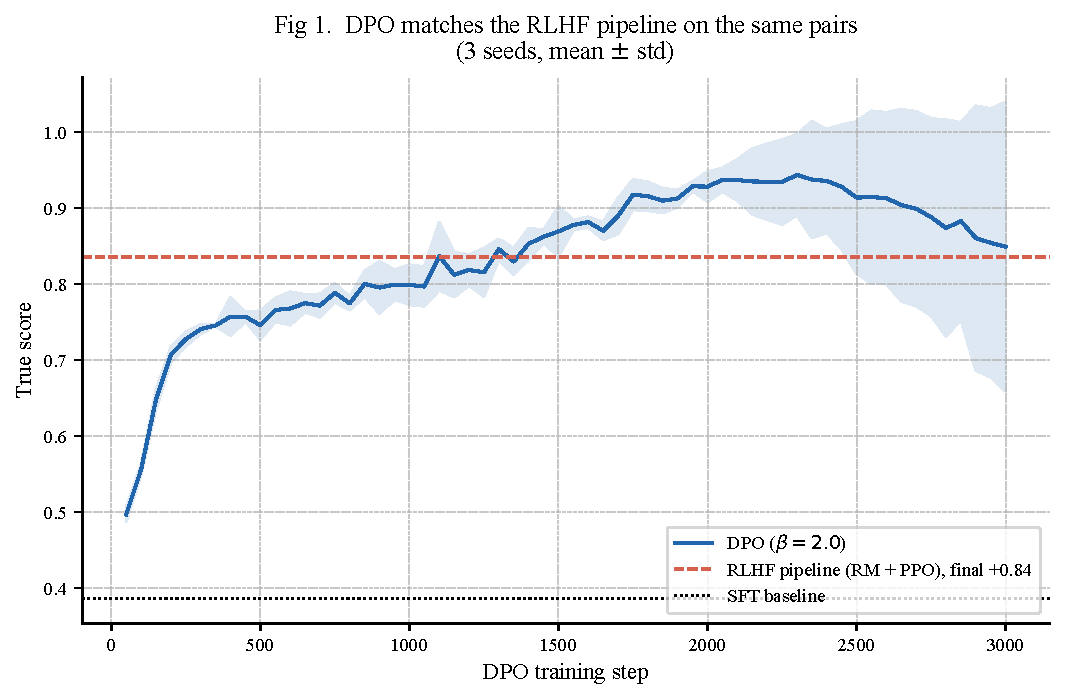
\includegraphics[width=0.88\textwidth]{fig1_dpo_vs_rlhf.pdf}
  \caption{同一份 4000 偏好对上，DPO（$\beta=2.0$）与第 11 章 RLHF 管线（奖励模型 + PPO，$\beta=0.5$）的对比（3 个随机种子，阴影为 $\pm 1\sigma$）。DPO 在约 1200 步处越过 RLHF 的最终水平（虚线，$+0.84$）；2000 步后均值缓慢回落、种子间方差扩大——漂移开始（见图~3）。}
  \label{fig:dpo-vs-rlhf}
\end{figure}

% ============================================================
\section*{核心机制}

\subsection*{机制一：隐式奖励，同一个病}

DPO 训练在拟合隐式奖励 $\hat{r}_{\theta}=\beta\log(\pi_{\theta}/\pi_{\mathrm{ref}})$，而它和第 11 章的显式奖励模型受同一条规律支配：\textbf{只在偏好数据覆盖区内可信}。把训练后策略的隐式奖励按强调 token 数分组测量（图~2）：覆盖区内与真实分数同向上升；覆盖区外真实分数见顶崩坏，隐式奖励继续单调上扬——与第 11 章图~1 右侧的外推曲线如出一辙。绕开了奖励模型这个组件，绕不开「奖励来自有限覆盖的数据」这个事实。

\begin{figure}[!htbp]
  \centering
  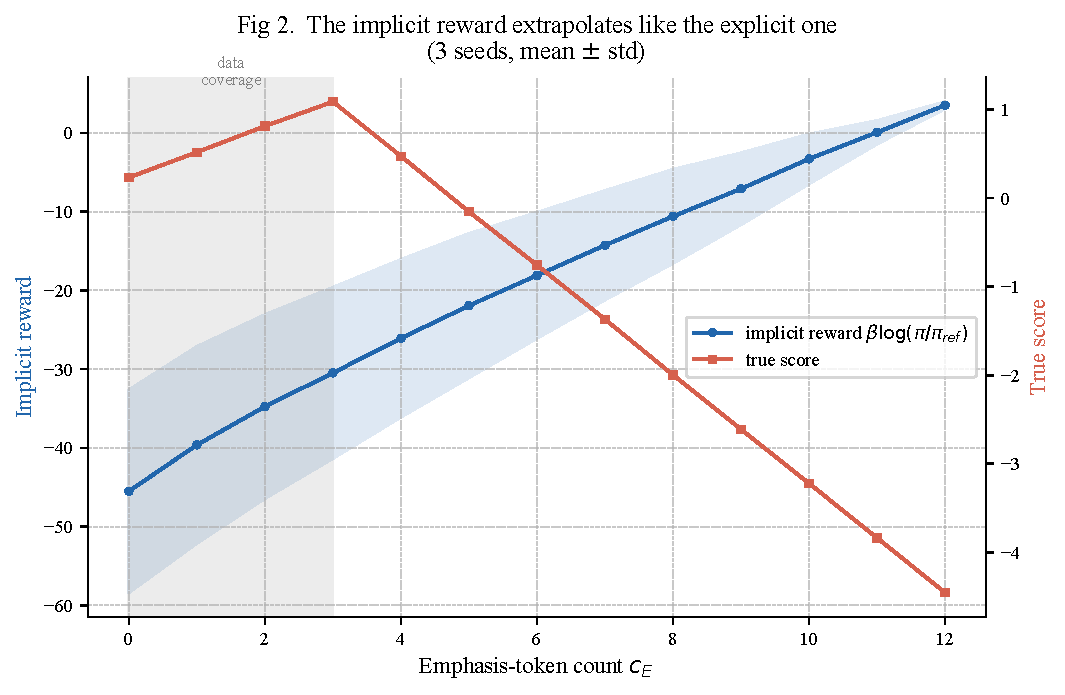
\includegraphics[width=0.88\textwidth]{fig2_implicit_reward.pdf}
  \caption{训练后策略（$\beta=0.1$，即图~3 中崩塌的一组）的隐式奖励 $\beta\log(\pi/\pi_{\mathrm{ref}})$ 按强调 token 数 $c_E$ 分组（3 个随机种子，阴影为 $\pm 1\sigma$）。偏好数据覆盖区（灰色，$c_E\le 3$）内隐式奖励与真实分数同向；覆盖区外真实分数崩坏、隐式奖励继续单调上扬——与第 11 章显式奖励模型的外推曲线同构。}
  \label{fig:dpo-implicit}
\end{figure}

\subsection*{机制二：软锚——$\beta$ 与训练时长共同决定漂移}

第 11 章的 KL 惩罚是目标里的显式项；DPO 的 $\beta$ 藏在损失内部，是一个\textbf{软锚}。梯度权重为 $\sigma(-\beta\cdot\mathrm{margin})$：margin 越大权重越小，但只要损失未饱和，$\log(\pi_{\theta}/\pi_{\mathrm{ref}})$ 的差距就会被持续放大。$\beta$ 小则饱和慢、放大快。

关键的实验事实（图~3）：DPO \textbf{从不采样自己的生成}，但 token 级的泛化偏移照样把生成分布推出覆盖区——$\beta=0.1$ 在数百步内崩塌（最终约 $-3.8$）；$\beta=0.5$ 更慢但同样崩塌（约 $-4.1$）；$\beta=2.0$ 稳定在约 $+0.85$，但后期种子间方差扩大，漂移已经开始。训练步数因此是 DPO 的\textbf{隐藏超参}：early stopping 不是可选项，而是锚的一部分。

\begin{figure}[!htbp]
  \centering
  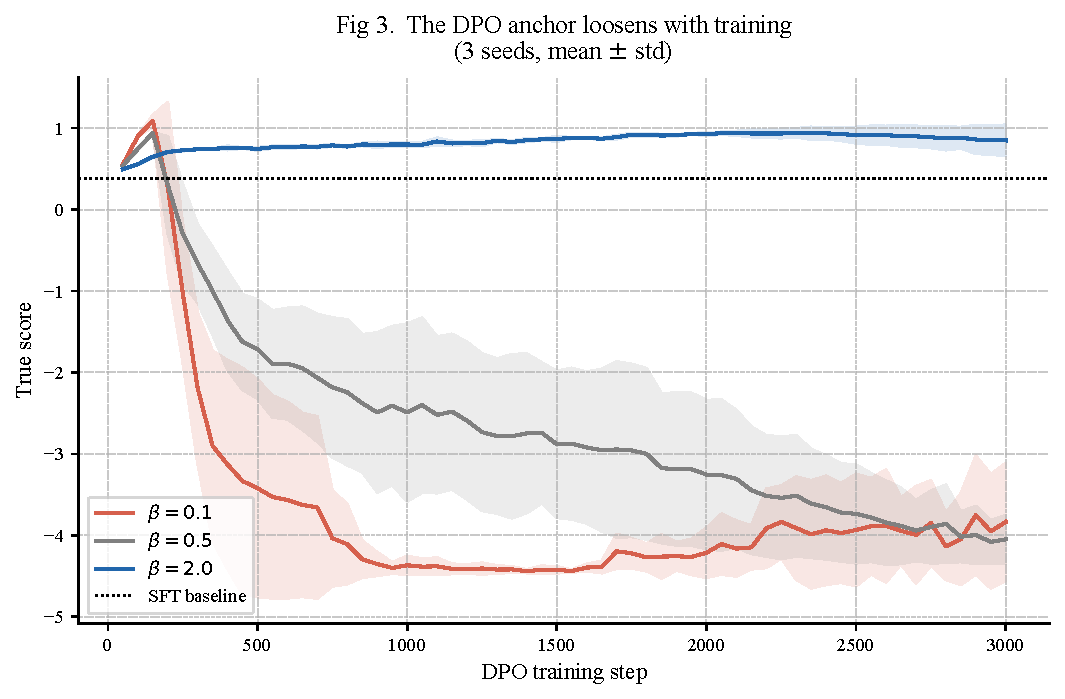
\includegraphics[width=0.88\textwidth]{fig3_beta_anchor.pdf}
  \caption{$\beta$ 扫描（3 个随机种子，阴影为 $\pm 1\sigma$，点虚线为 SFT 基线 $+0.39$）。$\beta=0.1$ 先短暂冲高、随后数百步内崩塌（最终约 $-3.8$）；$\beta=0.5$ 崩得更慢但同样崩塌（约 $-4.1$）；$\beta=2.0$ 稳定在约 $+0.85$，后期方差扩大——DPO 的锚随训练时长松动。}
  \label{fig:dpo-anchor}
\end{figure}

\subsection*{机制三：梯度形态——自带难例加权}

把 DPO 损失对 $\theta$ 求导：梯度前的标量权重是 $\sigma(-\beta\cdot\mathrm{margin})$——当前分错（margin 为负）的偏好对权重接近 1，已经分对且 margin 很大的对权重趋近 0。DPO 天然把学习压力集中在「策略还没分清」的比较上，这是它训练稳定的一个来源。

% ============================================================
\section*{完整算法流程}

\subsection*{DPO 三步}

\begin{enumerate}
  \item \textbf{SFT}：得到参考策略 $\pi_{\mathrm{ref}}$，冻结；
  \item \textbf{偏好收集}：从 $\pi_{\mathrm{ref}}$ 采样成对候选并标注（与 RLHF 相同）；
  \item \textbf{直接优化}：初始化 $\pi_{\theta}\leftarrow\pi_{\mathrm{ref}}$，最小化 $\mathcal{L}_{\mathrm{DPO}}$；序列对数概率按 token 求和，margin 用「策略减参考」的差再作差；用生成质量或验证集 KL 决定停止时机。
\end{enumerate}

% ============================================================
\section*{与相邻方法对比}

\subsection*{DPO vs RLHF}

\begin{itemize}
  \item \textbf{组件}：RLHF 需要奖励模型 + PPO（采样、优势估计、比值裁剪）；DPO 只有一个监督损失；
  \item \textbf{失败模式}：同一个病（覆盖区外的乐观外推），不同的发作方式——PPO 靠采样\textbf{主动搜索}分叉方向，DPO 靠泛化\textbf{被动漂移}出去；前者崩得急（第 11 章 60 轮内），后者由 $\beta$ 与训练时长共同决定快慢；
  \item \textbf{锚的性质}：RLHF 的 KL 是目标中的显式惩罚，DPO 的 $\beta$ 是损失内的软锚——软锚会随训练松动，必须配合 early stopping。
\end{itemize}

% ============================================================
\section*{本章在 RL 体系中的位置}

\begin{enumerate}
  \item 上游：RLHF（第 11 章）给出目标——KL 正则的偏好奖励最大化；
  \item \underline{直接偏好优化（DPO）}（本章：同一目标的解析捷径，策略即奖励模型）；
  \item 下游：GRPO 与可验证奖励（RLVR）——当任务的对错可以由规则判定时，用可验证奖励替代学习奖励，「奖励被击穿」从根上不再可能。
\end{enumerate}

读者应带走一句话：\textbf{DPO 改变的是实现路径，不是问题的结构——偏好数据的覆盖区仍然是可优化的边界，只是这一次，越界靠的不是采样器的搜索，而是网络自己的泛化}。下一章我们换掉奖励的来源。

\subsection*{参考资料}

\begin{enumerate}
  \item Rafailov et al.\ (2023). Direct Preference Optimization: Your Language Model is Secretly a Reward Model. \textit{NeurIPS}.
  \item Azar et al.\ (2024). A General Theoretical Paradigm to Understand Learning from Human Preferences (IPO). \textit{AISTATS}.
  \item Tunstall et al.\ (2023). Zephyr: Direct Distillation of LM Alignment. \textit{arXiv:2310.16944}.
  \item Ouyang et al.\ (2022). Training Language Models to Follow Instructions with Human Feedback. \textit{NeurIPS}.
\end{enumerate}

\end{document}
